% !TeX program = xelatex
% !TeX encoding = UTF-8
% !TeX TXS-program:compile = txs:///xelatex | txs:///xelatex
\documentclass[aspectratio=169, table, 12pt]{beamer}

% Preamble bersama seluruh slide mata kuliah ini.
% Dipanggil dari slides/sessionXX/sessionXX.tex tepat sesudah baris
% \documentclass[aspectratio=169, table, 12pt]{beamer}
% Paket tambahan yang hanya dibutuhkan satu sesi ditulis di berkas sesi itu.

\usepackage{colortbl}
\usepackage{xcolor}
\usepackage{listings}
\usepackage{tabularx}
\usepackage{booktabs}
\usepackage{tikz}
\usepackage{pgfplots}
\usepackage{fontspec}
\usepackage[english,bahasai]{babel}
\pgfplotsset{compat=1.18}
\usetikzlibrary{arrows.meta, positioning, calc, fit, shapes.geometric,
  shapes.multipart, backgrounds, matrix, chains, trees}

\makeatletter
\def\input@path{{../theme/}}
\makeatother
\graphicspath{{../theme/}{../../figures/}}
% Stub symlink Windows memakai tema cadangan sampai aset institusi tersedia.
\IfFileExists{../theme/beamerthemePradita.sty}{%
  \usetheme{Pradita}
}{%
  \usetheme{Madrid}
  \setmainfont{TeX Gyre Heros}
  \setsansfont{TeX Gyre Heros}
  \setbeamertemplate{navigation symbols}{}
}

\definecolor{praditagreen}{RGB}{37, 113, 71}
\setbeamercolor{structure}{fg=praditagreen}
\setbeamercolor{palette primary}{bg=praditagreen,fg=white}
\setbeamercolor{palette secondary}{bg=praditagreen!80!black,fg=white}
\setbeamercolor{palette tertiary}{bg=praditagreen!60!black,fg=white}
\setbeamerfont{frametitle}{size=\large}
\setbeamertemplate{caption}[numbered]

% Ukuran header mengikuti teks agar judul panjang tidak menabrak logo.
\setbeamercolor{frametitle}{bg=white,fg=black}
\setbeamertemplate{frametitle}{%
  \begin{beamercolorbox}[wd=\paperwidth,sep=0.2cm]{frametitle}
    \begin{minipage}[c]{0.77\paperwidth}
      \raggedright\fontsize{16}{18}\selectfont\bfseries\insertframetitle
      \ifx\insertframesubtitle\empty\else
        \par\small\mdseries\insertframesubtitle
      \fi
    \end{minipage}\hfill
    \begin{minipage}[c]{0.15\paperwidth}
      \IfFileExists{../theme/classFiles/logo_universitas.png}{%
        
\includegraphics[width=\linewidth]{../theme/classFiles/logo_universitas.png}%
      }{}
    \end{minipage}
  \end{beamercolorbox}
}
\setbeamertemplate{footline}{%
  \ifnum\value{framenumber}>1
    \begin{beamercolorbox}[wd=\paperwidth,ht=0.35cm,dp=0.15cm,
      leftskip=0.3cm,rightskip=0.3cm]{palette primary}
      \footnotesize\bfseries\insertframenumber/\inserttotalframenumber
      \hfill IT40813
    \end{beamercolorbox}
  \fi
}
\DeclareRobustCommand{\berkas}[1]{\path{#1}}

% Tema membuat garis tabel berwarna putih. Dikembalikan agar tabel terbaca.
\arrayrulecolor{black}
\setlength{\arrayrulewidth}{0.5pt}

\lstdefinelanguage{yaml}{
  basicstyle=\ttfamily\scriptsize,
  keywordstyle=\color{blue}\bfseries,
  commentstyle=\color{gray}\itshape,
  stringstyle=\color{red},
  showstringspaces=false,
  breaklines=true,
  frame=lines,
  numbers=none,
  backgroundcolor=\color{lightgray!10},
  tabsize=2,
  morecomment=[l]{\#}
}

\lstdefinelanguage{json}{
  basicstyle=\ttfamily\scriptsize,
  stringstyle=\color{red},
  commentstyle=\color{gray},
  breaklines=true,
  showstringspaces=false,
  tabsize=2,
  numbers=none,
  frame=lines,
  backgroundcolor=\color{lightgray!10},
  string=[s]{"}{"}
}

\lstdefinelanguage{bash}{
  keywords={},
  basicstyle=\ttfamily\scriptsize,
  ndkeywords={docker, kubectl, helm, curl, git, terraform},
  ndkeywordstyle=\color{purple}\bfseries,
  sensitive=true,
  commentstyle=\color{gray},
  numbers=none,
  breaklines=true,
  frame=lines,
  backgroundcolor=\color{lightgray!10},
  tabsize=2,
  comment=[l]{\#},
  showstringspaces=false
}

\lstdefinelanguage{http}{
  keywords={GET, POST, PUT, PATCH, DELETE, HEAD, OPTIONS, HTTP},
  basicstyle=\ttfamily\scriptsize,
  keywordstyle=\color{blue}\bfseries,
  sensitive=true,
  numbers=none,
  breaklines=true,
  frame=lines,
  backgroundcolor=\color{lightgray!10},
  tabsize=2,
  showstringspaces=false
}

\subtitle{IT40813 · IT Governance, Risk \& Compliance}
\author{\textbf{Alfa Yohannis}}


% Sampul membatasi judul di panel putih tema rujukan Pradita.
\setbeamertemplate{title page}{%
  \begin{tikzpicture}[remember picture,overlay]
    \node[anchor=north west,inner sep=0pt,text width=8.8cm]
      at ([xshift=1cm,yshift=-3.15cm]current page.north west) {%
        {\small\insertsubtitle\par}\vspace{0.25cm}
        \resizebox{8.8cm}{!}{\begin{minipage}{12cm}
          \raggedright\color{praditagreen}\bfseries\inserttitle
        \end{minipage}}
      };
    \node[anchor=south west,inner sep=0pt]
      at ([xshift=1cm,yshift=1.65cm]current page.south west)
      {\small\insertdate};
    \node[anchor=west,inner sep=0pt,text=white]
      at ([xshift=0.8cm,yshift=0.75cm]current page.south west)
      {\small\insertauthor};
  \end{tikzpicture}
}


\title{\Huge Tata Kelola\\ \vspace{10pt} Kecerdasan Artifisial}
\date{Pertemuan 11}

\begin{document}

\frame{\titlepage}

\begin{frame}
  \frametitle{Isi Pertemuan}
  \vspace{14pt}
  \begin{columns}[t]
    \column{0.5\textwidth}
    {\small\tableofcontents[sections={1-4}]}

    \column{0.5\textwidth}
    {\small\tableofcontents[sections={5-8}]}
  \end{columns}
\end{frame}

\begin{frame}{\hfill}
  \centering
  \Huge{\textbf{Ringkasan 12 menit selesai cepat.\\Siapa menjawab bila\\alergi pasien hilang?}}
\end{frame}

\section{Tujuan dan Konteks}

\begin{frame}{{\Large Tujuan Pembelajaran}}
  \vspace{10pt}
  \begin{itemize}
    \item Mengidentifikasi kasus pemakaian AI (\textit{Artificial Intelligence}) di organisasi dan
          mengklasifikasi risikonya.
    \item Menjelaskan persyaratan sistem manajemen AI menurut ISO/IEC 42001:2023 dan pendekatan
          berbasis risiko dalam EU AI Act.
    \item Merumuskan kebijakan pemakaian AI yang dapat dijalankan dan diawasi.
  \end{itemize}
\end{frame}

\begin{frame}{{\Large Masalah: Keputusan AI Sudah Terjadi}}
  \vspace{6pt}
  \small
  \begin{itemize}
    \item Misalkan petugas memakai \textit{chatbot} AI umum untuk merangkum catatan pasien, tanpa
          izin.
    \item Lokasi teks, pemakaian ulang oleh penyedia, dan ketepatan ringkasan tidak diketahui.
    \item Medikara belum punya proyek AI resmi, tetapi keputusan data dan keselamatan sudah terjadi.
    \item Kesalahan pengelompokan surat tidak berakibat sama dengan kesalahan triase.
    \item Hasil kerja: inventaris AI dan kebijakan pemakaian AI untuk tonggak C3.
  \end{itemize}
\end{frame}

\begin{frame}{{\Large Diagram Konsep Bab 11}}
  \centering
  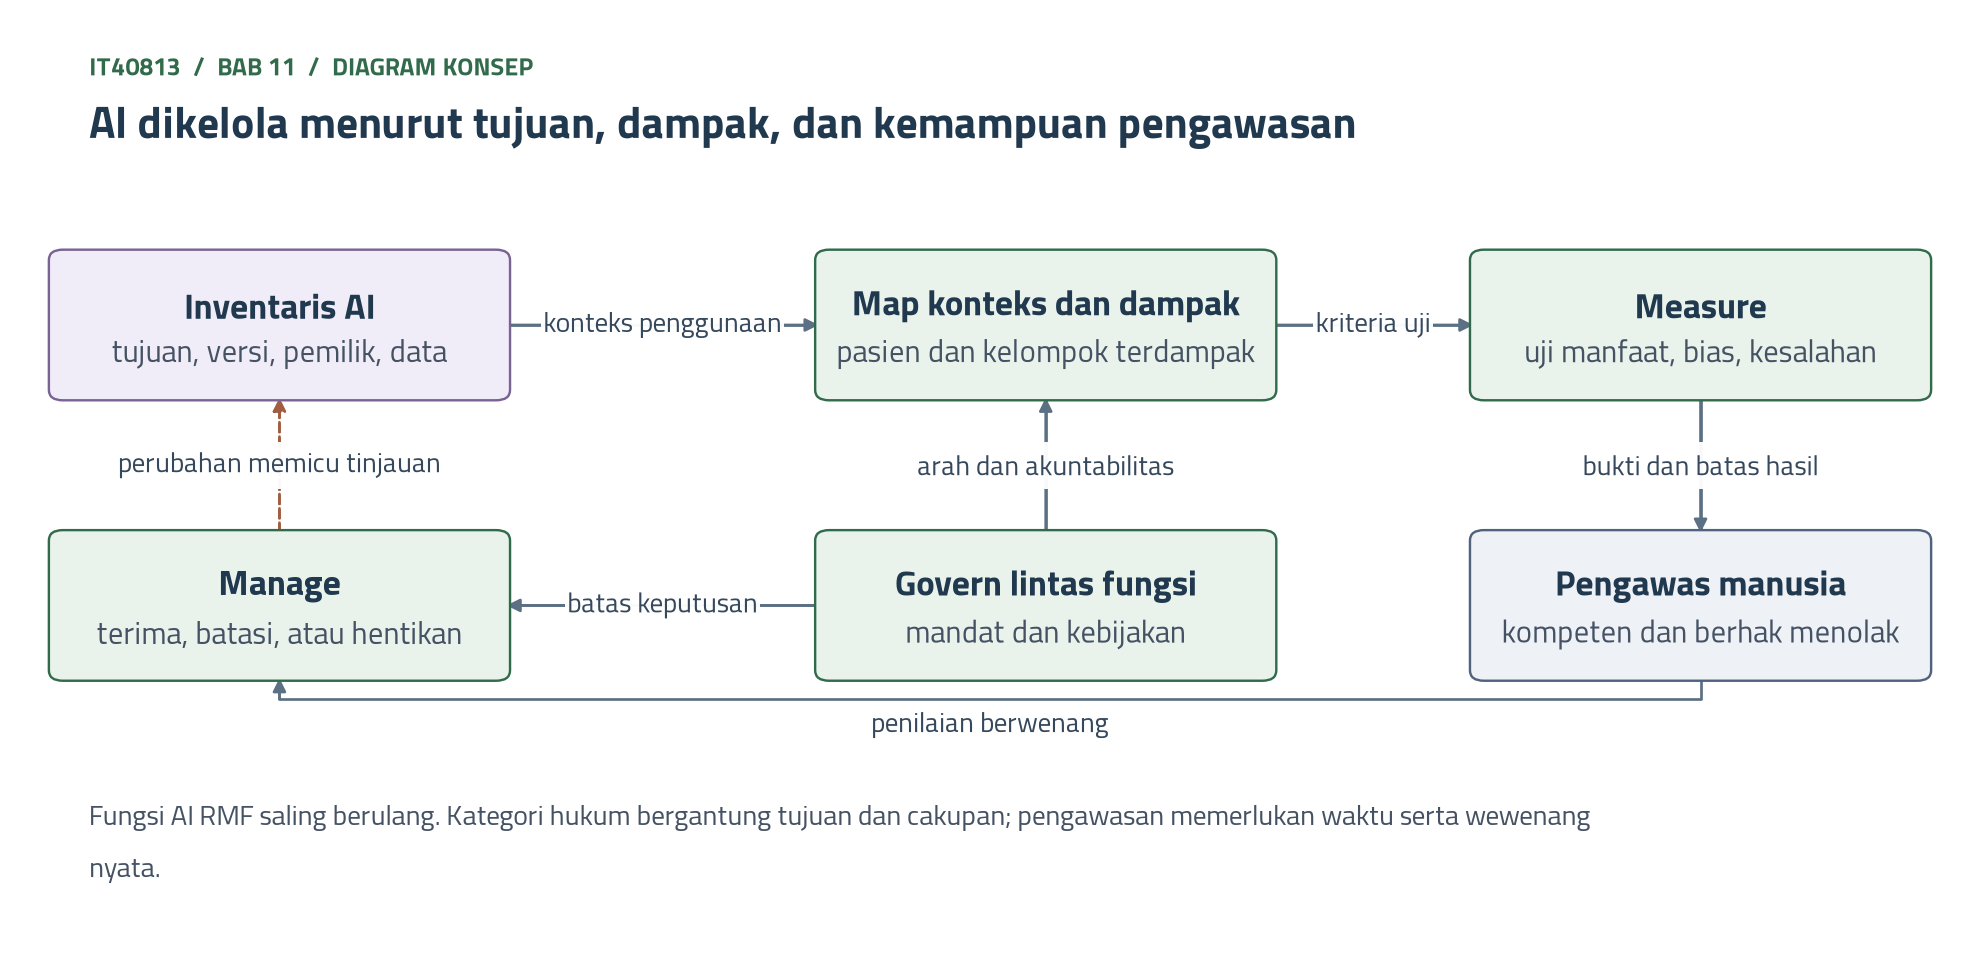
\includegraphics[width=0.96\textwidth,height=0.77\textheight,keepaspectratio]{../../figures/ch11-diagram-konsep.png}
  \label{fig:session11-ilustrasi-bab}
\end{frame}

\section{Peluang dan Risiko}

\begin{frame}{{\Large Enam Kasus Pemakaian (Misalkan)}}
  \vspace{2pt}
  \scriptsize
  \begin{tabularx}{\textwidth}{|>{\raggedright\arraybackslash}p{0.09\textwidth}|>{\raggedright\arraybackslash}X|>{\raggedright\arraybackslash}X|>{\raggedright\arraybackslash}X|}
    \hline
    \textbf{Kode} & \textbf{Kasus} & \textbf{Manfaat yang diuji} & \textbf{Risiko utama} \\ \hline
    AI-01 & Ringkasan rekam medis & Waktu dokumentasi & Alergi atau obat terlewat \\ \hline
    AI-02 & Prioritas triase darurat & Waktu sampai ditangani & Kasus gawat diberi prioritas
    rendah \\ \hline
    AI-03 & Prediksi tempat tidur & Ketepatan perencanaan & Kinerja berubah antarperiode dan
    antarlokasi \\ \hline
    AI-04 & Deteksi kecurangan klaim & Prioritas pemeriksaan & Tuduhan salah dan bias \\ \hline
    AI-05 & Informasi gejala umum di Medikara+ & Pertanyaan terjawab tanpa antre & Jawaban keliru
    dibaca sebagai nasihat medis \\ \hline
    AI-06 & \textit{Chatbot} umum tanpa izin & Tidak diukur & Data pasien keluar tanpa kendali \\
    \hline
  \end{tabularx}

  \vspace{6pt}
  \small Analogi asisten baru: draf cepat, tetapi belum berwenang memutuskan pengobatan.
\end{frame}

\begin{frame}{{\Large Manfaat Bersih: Klaim dan Hasil Uji}}
  \vspace{4pt}
  \begin{center}
    \resizebox{0.92\textwidth}{!}{\begin{tikzpicture}[
  x=0.47cm, y=0.72cm,
  font=\scriptsize,
  label/.style={anchor=east, align=right},
  hasil/.style={anchor=west, align=left, text width=2.5cm},
  isi/.style={midway, font=\scriptsize}]
  % Baris 1: penulisan manual sebagai ukuran awal.
  \node[label] at (0,3.5) {Manual\\(ukuran awal)};
  \draw[fill=blue!8] (0,3.2) rectangle (12,3.8) node[isi] {Menulis 12};
  \node[hasil] at (14.3,3.5) {12 menit};
  % Baris 2: klaim vendor mengabaikan waktu pemeriksaan.
  \node[label] at (0,2.5) {Klaim vendor};
  \draw[fill=green!10] (0,2.2) rectangle (2,2.8) node[isi] {Draf 2};
  \node[hasil] at (14.3,2.5) {Klaim hemat 10};
  % Baris 3: hasil uji dengan pemeriksaan 8 menit.
  \node[label] at (0,1.5) {Hasil uji\\(periksa 8 menit)};
  \draw[fill=green!10] (0,1.2) rectangle (2,1.8) node[isi] {Draf 2};
  \draw[fill=orange!12] (2,1.2) rectangle (10,1.8) node[isi] {Periksa 8};
  \node[hasil] at (14.3,1.5) {Hemat 2};
  % Baris 4: pemeriksaan lebih panjang menghapus penghematan.
  \node[label] at (0,0.5) {Diperpanjang\\(periksa 12 menit)};
  \draw[fill=green!10] (0,0.2) rectangle (2,0.8) node[isi] {Draf 2};
  \draw[fill=red!22] (2,0.2) rectangle (14,0.8) node[isi] {Periksa 12};
  \node[hasil] at (14.3,0.5) {Lebih lama 2};
  % Sumbu waktu dan batas manual.
  \draw[-{Stealth[length=2mm]}, thick] (0,0) -- (14.6,0);
  \foreach \menit in {0,2,4,6,8,10,12,14} {
    \draw (\menit,0) -- (\menit,-0.1) node[below] {\menit};
  }
  \draw[dashed, thick] (12,0) -- (12,4.1) node[above] {Batas manual};
  \node[below=3.5mm] at (7,0) {Menit per ringkasan (misalkan)};
\end{tikzpicture}
}
  \end{center}
  \small Pemeriksaan menghapus sebagian besar penghematan yang diklaim.
\end{frame}

\begin{frame}{{\Large Hitungan pada 60.000 Ringkasan per Tahun}}
  \vspace{6pt}
  \small
  \begin{itemize}
    \item Tarif Rp60.000 per jam dari Bab 7, atau Rp1.000 per menit.
    \item Klaim hemat 10 menit: 10.000 jam, senilai Rp600 juta per tahun.
    \item Hasil uji hemat 2 menit: 2.000 jam, senilai Rp120 juta. Dengan lisensi Rp150 juta,
          manfaat bersihnya minus Rp30 juta. Titik impasnya 2,5 menit.
    \item Pada tarif dokter Rp150.000 per jam, manfaat bersihnya Rp150 juta. Titik impas tarif
          Rp75.000 per jam.
    \item Memotong waktu pemeriksaan memenuhi hitungan, tetapi melemahkan pengawasan.
  \end{itemize}
\end{frame}

\begin{frame}{{\Large Shadow AI}}
  \vspace{6pt}
  \small
  \begin{itemize}
    \item \textit{Shadow AI}: pemakaian AI yang tidak tercatat atau di luar pengawasan organisasi.
    \item Analogi jalan setapak: papan larangan tidak menghapus kebutuhan. Buka jalur aman, lalu
          tutup jalan pintas yang berbahaya.
    \item Misalkan survei: 96 dari 600 responden (16 persen) memakai AI umum; 24 (4 persen)
          memasukkan data pasien.
    \item Disamaratakan ke 4.800 karyawan: sekitar 768 dan 192 orang. Perkiraan kasar, responden
          tidak acak.
    \item Laporan naik dari 2 menjadi 15 per bulan belum tentu berarti pelanggaran naik.
  \end{itemize}
\end{frame}

\begin{frame}{{\Large Kasus Medikara: 40 Catatan di Chatbot Umum}}
  \vspace{6pt}
  \small
  \begin{itemize}
    \item Misalkan kepala ruang mengetahui pada Selasa 10.00 bahwa 40 catatan telah diunggah.
    \item Fungsi hukum dan petugas pelindungan data menilai apakah ini kegagalan pelindungan data.
    \item Bila ya: batas internal jam ke-60 Kamis 22.00, batas terluar $3 \times 24$ jam Jumat
          10.00.
    \item Pertanyaan data: Pasal 966 dan Pasal 972 PP 28/2024. Pertanyaan keselamatan: apakah
          ringkasan masuk ke rekam medis?
    \item Sanksi saja tidak cukup. Peristiwa ini juga bukti kebutuhan kerja yang belum terpenuhi.
  \end{itemize}
\end{frame}

\begin{frame}{{\Large Kaitan dengan R-11 dan Urutan Keputusan}}
  \vspace{2pt}
  \begin{center}
    \resizebox{0.86\textwidth}{!}{\begin{tikzpicture}[
  node distance=5mm,
  font=\scriptsize,
  kotak/.style={draw, rounded corners, align=center, text width=2.4cm, minimum height=1cm},
  catatan/.style={align=center, text width=2.4cm},
  panah/.style={-{Stealth[length=2mm]}, thick}]
  \node[kotak, fill=praditagreen!15] (t0) {\textbf{Tujuan dan konteks}};
  \node[kotak, fill=blue!8, right=of t0] (t1) {\textbf{Dampak dan risiko}};
  \node[kotak, fill=orange!12, right=of t1] (t2) {\textbf{Batas pemakaian}};
  \node[kotak, fill=green!10, right=of t2] (t3) {\textbf{Evaluasi dan pengawasan}};
  \draw[panah] (t0) -- (t1);
  \draw[panah] (t1) -- (t2);
  \draw[panah] (t2) -- (t3);
  \node[catatan, below=2mm of t0] (c0)
    {Apa yang dibantu\\dan siapa\\memakainya?\\{\tiny\mdseries Bukti: baris inventaris}};
  \node[catatan, below=2mm of t1] (c1)
    {Siapa dirugikan bila keluaran salah?\\{\tiny\mdseries Bukti: penilaian dampak}};
  \node[catatan, below=2mm of t2] (c2)
    {Diizinkan, perlu persetujuan, atau ditahan?\\{\tiny\mdseries Bukti: kebijakan KB-09}};
  \node[catatan, below=2mm of t3] (c3)
    {Manfaat terbukti dan keluaran dapat ditolak?\\{\tiny\mdseries Bukti: hasil uji dan log}};
  \draw[panah, dashed] (c3.south) -- ++(0,-5mm) -| (c0.south)
    node[pos=0.25, below] {Perubahan tujuan, model, data, atau vendor memicu tinjauan ulang};
\end{tikzpicture}
}
  \end{center}
  \vspace{-4pt}
  \footnotesize
  \begin{itemize}
    \item R-11 tetap: skor $3 \times 4 = 12$, pemilik direktur pelayanan. Register tidak mendapat
          kode baru.
    \item AI-01 menambah jalur penyebab: alergi tercatat di sumber, tetapi hilang pada ringkasan.
    \item Kesalahan kritis masuk ke pimpinan klinis pada hari yang sama, seperti Bab 5.
  \end{itemize}
\end{frame}

\begin{frame}{{\Large Membaca Tiga Penelitian}}
  \vspace{2pt}
  \scriptsize
  \begin{tabularx}{\textwidth}{|>{\raggedright\arraybackslash}p{0.17\textwidth}|>{\raggedright\arraybackslash}X|>{\raggedright\arraybackslash}p{0.25\textwidth}|}
    \hline
    \textbf{Penelitian} & \textbf{Temuan} & \textbf{Pertanyaan bagi Medikara} \\ \hline
    Obermeyer dan rekan (2019) & Algoritma memprediksi biaya, bukan keparahan. Perbaikan bias
    menaikkan porsi pasien kulit hitam yang dibantu dari 17,7 menjadi 46,5 persen. & Apa yang
    diprediksi model? \\ \hline
    Wong dan rekan (2021) & Model sepsis pada 38.455 rawat inap: kemampuan membedakan 0,63;
    peringatan 18 persen; 1.709 dari 2.552 pasien sepsis (67 persen) tidak teridentifikasi. &
    Apakah kinerja bertahan di rumah sakit sendiri? \\ \hline
    Asgari dan rekan (2025) & 12.999 kalimat beranotasi klinisi: halusinasi 1,47 persen,
    penghilangan 3,45 persen. & Kesalahan jenis apa, dan apa pembandingnya? \\ \hline
  \end{tabularx}

  \vspace{6pt}
  \small Hitungan bab: sekitar 8 peringatan per satu kasus sepsis pada penelitian Wong. Angka
  penelitian tidak disalin menjadi perkiraan Medikara.
\end{frame}

\section{ISO/IEC 42001}

\begin{frame}{{\Large Sistem Manajemen AI}}
  \vspace{6pt}
  \small
  \begin{itemize}
    \item ISO/IEC 42001 menetapkan persyaratan: konteks, kepemimpinan, perencanaan, dukungan,
          operasi, evaluasi, dan perbaikan.
    \item Yang khas: penilaian risiko AI dan penilaian dampak sistem AI.
    \item Analogi alat laboratorium: sistem memastikan pemilik dan prosedur, bukan setiap hasil
          benar.
    \item Misalkan 2 dari 10 model masuk ruang lingkup. Bukti 20 persen itu bukan klaim seluruh
          portofolio.
    \item Naskah berbayar. Nomor klausul diambil dari \textit{crosswalk} NIST ke rancangan akhir
          standar, dan perlu dicocokkan.
  \end{itemize}
\end{frame}

\begin{frame}{{\Large Klausul pada AI-01 (Misalkan)}}
  \vspace{2pt}
  \scriptsize
  \begin{tabularx}{\textwidth}{|>{\raggedright\arraybackslash}p{0.27\textwidth}|>{\raggedright\arraybackslash}X|>{\raggedright\arraybackslash}X|}
    \hline
    \textbf{Klausul} & \textbf{Pertanyaan} & \textbf{Bukti pada AI-01} \\ \hline
    4.1 Konteks & Apa yang tercakup? & Satu rumah sakit tahap uji; UU PDP, PP 28/2024 \\ \hline
    5.1 sampai 5.3 Kepemimpinan & Siapa menetapkan? & KB-09; direktur pelayanan pemilik \\ \hline
    6.1.2 dan 6.1.3 Risiko AI & Apa yang diperlakukan? & R-11 skor 12; alergi dari data terstruktur
    \\ \hline
    6.1.4 Dampak sistem AI & Siapa terdampak? & Penilaian 72 jam; pasien lanjut usia \\ \hline
    7.2 Kompetensi & Apakah pemeriksa mampu? & 120 dokter dilatih 2 jam \\ \hline
    8.2 sampai 8.4 Operasi & Dijalankan saat berubah? & Inventaris diperbarui; uji diulang \\ \hline
    9.1 dan 9.3 Evaluasi & Dipantau dan ditinjau? & 4 dari 100; agenda komite risiko \\ \hline
    10.1 Perbaikan & Apa yang berubah? & Rancangan diubah; uji ulang 1 dari 100 \\ \hline
  \end{tabularx}
\end{frame}

\begin{frame}{{\Large Penilaian Dampak dan Penilaian Risiko}}
  \vspace{6pt}
  \small
  \begin{itemize}
    \item Penilaian risiko: akibat terhadap tujuan organisasi. Penilaian dampak: akibat bagi
          individu, kelompok, dan masyarakat.
    \item Analogi jalan di depan pasar: aman bagi kontraktor, tetapi merugikan pedagang.
    \item AI-04: pemeriksaan 300 tanda per bulan hanya 100 jam atau Rp6 juta, tetapi 93 dari 120
          tanda pada klinik keliru.
    \item Beban penilaian: 72, 72, 24, 24, dan 8 jam, jumlah 200 jam atau Rp12 juta.
    \item AI-01 dan AI-02 digabung dengan DPIA agar tidak ada dua dokumen untuk data yang sama.
  \end{itemize}
\end{frame}

\begin{frame}{{\Large AI dan Keamanan Informasi}}
  \vspace{4pt}
  \footnotesize
  \begin{tabularx}{\textwidth}{|>{\raggedright\arraybackslash}X|>{\raggedright\arraybackslash}X|>{\raggedright\arraybackslash}X|}
    \hline
    \textbf{Acuan} & \textbf{Fokus} & \textbf{Bukti contoh} \\ \hline
    ISO/IEC 42001 & Pengelolaan AI bertanggung jawab & Kebijakan, evaluasi, tindak lanjut \\ \hline
    ISO/IEC 42005 & Dampak penggunaan AI & Pihak terdampak dan mitigasi \\ \hline
    ISO/IEC 27001 & Risiko keamanan informasi & Kontrol akses dan insiden \\ \hline
  \end{tabularx}

  \vspace{8pt}
  \small Sertifikasi salah satunya tidak otomatis memenuhi yang lain, dan tidak membuktikan
  kepatuhan hukum atau kebenaran setiap keluaran AI.
\end{frame}

\section{NIST AI RMF}

\begin{frame}{{\Large Empat Fungsi pada AI-01 (Misalkan)}}
  \vspace{2pt}
  \scriptsize
  \begin{tabularx}{\textwidth}{|>{\raggedright\arraybackslash}p{0.13\textwidth}|>{\raggedright\arraybackslash}X|>{\raggedright\arraybackslash}X|>{\raggedright\arraybackslash}X|}
    \hline
    \textbf{Fungsi} & \textbf{Pertanyaan} & \textbf{Bukti} & \textbf{Pada AI-01} \\ \hline
    Govern & Siapa bertanggung jawab? & Pemilik dan batas keputusan & Direktur pelayanan; KB-09 \\
    \hline
    Map & Siapa dapat dirugikan? & Konteks dan pihak terdampak & Pasien dengan alergi; pasien
    lanjut usia \\ \hline
    Measure & Risikonya terbukti bagaimana? & Hasil uji per kelompok & 100 kasus sintetis, dua
    penilai \\ \hline
    Manage & Kapan dihentikan atau diperbaiki? & Keputusan dan pemicu tinjauan & Ditahan; alergi
    ditarik dari data terstruktur \\ \hline
  \end{tabularx}

  \vspace{6pt}
  \small Kerangka sukarela. Tindakannya bukan daftar periksa atau urutan tetap. Govern bekerja
  lintas fungsi, dan perubahan memicu tinjauan.
\end{frame}

\begin{frame}{{\Large Measure: Satu Angka Sering Menyesatkan}}
  \vspace{6pt}
  \small
  \begin{itemize}
    \item Analogi alarm rusak: benar 364 hari, gagal pada satu hari kebakaran.
    \item Misalkan 1.500 sesi per bulan, 30 sesi (2 persen) benar-benar darurat.
    \item Model yang selalu menjawab ``bukan darurat'': ketepatan 98 persen, melewatkan 30 kasus.
    \item Model lain: 27 dari 30 tertangkap, sekitar 74 sesi salah tanda, ketepatan 94,9 persen.
    \item Sisa 3 kasus per bulan, atau 36 per tahun, tetap harus dijawab jalur lain.
  \end{itemize}
\end{frame}

\begin{frame}{{\Large Uji AI-01 per Kelompok (Misalkan)}}
  \vspace{2pt}
  \footnotesize
  \begin{tabularx}{\textwidth}{|>{\raggedright\arraybackslash}X|>{\raggedright\arraybackslash}p{0.1\textwidth}|>{\raggedright\arraybackslash}p{0.16\textwidth}|>{\raggedright\arraybackslash}p{0.12\textwidth}|>{\raggedright\arraybackslash}p{0.16\textwidth}|>{\raggedright\arraybackslash}p{0.12\textwidth}|}
    \hline
    \textbf{Kelompok} & \textbf{Kasus} & \textbf{Putaran 1} & \textbf{Persen} & \textbf{Putaran 2} &
    \textbf{Persen} \\ \hline
    Di bawah 60 tahun & 60 & 1 & 1,7 & 0 & 0 \\ \hline
    60 tahun ke atas & 40 & 3 & 7,5 & 1 & 2,5 \\ \hline
    Seluruh kasus & 100 & 4 & 4,0 & 1 & 1,0 \\ \hline
  \end{tabularx}

  \vspace{6pt}
  \small
  \begin{itemize}
    \item Kriteria ditetapkan lebih dahulu: tidak melebihi manual 1 persen; tiap kelompok paling
          tinggi 3 persen.
    \item Perubahan: alergi dan obat ditarik dari data terstruktur, bukan ditulis model.
    \item Keputusan: batasi, bukan terima. Sampel kecil hanya membuka tahap berikutnya.
  \end{itemize}
\end{frame}

\begin{frame}{{\Large Deteksi Klaim AI-04 per Sumber (Misalkan)}}
  \vspace{2pt}
  \footnotesize
  \begin{tabularx}{\textwidth}{|>{\raggedright\arraybackslash}X|>{\raggedright\arraybackslash}p{0.1\textwidth}|>{\raggedright\arraybackslash}p{0.17\textwidth}|>{\raggedright\arraybackslash}p{0.17\textwidth}|>{\raggedright\arraybackslash}p{0.17\textwidth}|}
    \hline
    \textbf{Sumber} & \textbf{Klaim} & \textbf{Ditandai} & \textbf{Terbukti} & \textbf{Tanda keliru}
    \\ \hline
    Rumah sakit & 4.500 & 180 (4 persen) & 63 (35 persen) & 117 (65 persen) \\ \hline
    Klinik & 1.500 & 120 (8 persen) & 27 (22,5 persen) & 93 (77,5 persen) \\ \hline
    Jumlah & 6.000 & 300 (5 persen) & 90 (30 persen) & 210 (70 persen) \\ \hline
  \end{tabularx}

  \vspace{8pt}
  \small Klinik ditandai dua kali lebih sering, tetapi tandanya lebih sering keliru. Presisi total
  30 persen menutupi kesenjangan itu. Pertanyaan Obermeyer berlaku: apa yang diukur model?
\end{frame}

\begin{frame}{{\Large Profil AI Generatif: Lima dari 12 Risiko}}
  \vspace{6pt}
  \small
  \begin{itemize}
    \item Confabulation: AI-01 menulis obat yang tidak diresepkan.
    \item Data Privacy: AI-06, catatan pasien pada \textit{chatbot} umum.
    \item Harmful Bias or Homogenization: AI-01 lebih sering salah pada pasien lanjut usia.
    \item Human-AI Configuration: pemeriksa setuju tanpa membaca sumber.
    \item Value Chain and Component Integration: vendor mengganti model tanpa pemberitahuan. Bab 9
          memberi pegangan 30 hari.
  \end{itemize}
\end{frame}

\section{EU AI Act}

\begin{frame}{{\Large Urutan Pertanyaan Klasifikasi}}
  \vspace{-2pt}
  \begin{center}
    \resizebox{!}{0.77\textheight}{\begin{tikzpicture}[
  font=\scriptsize,
  tanya/.style={draw, rounded corners, align=left, text width=6.9cm, minimum height=0.95cm},
  hasil/.style={draw, rounded corners, align=center, text width=3.1cm, minimum height=0.95cm},
  panah/.style={-{Stealth[length=2mm]}, thick},
  ket/.style={midway, font=\tiny, fill=white, inner sep=1pt}]
  \node[tanya, fill=praditagreen!15] (q0) at (0,0)
    {\textbf{Article 2, 3, dan 25.} Apakah organisasi tercakup, dan apa perannya: penyedia atau
    penerap?};
  \node[tanya, fill=blue!8] (q1) at (0,-1.5)
    {\textbf{Article 5.} Apakah pemakaian termasuk praktik terlarang?};
  \node[tanya, fill=blue!8] (q2) at (0,-3)
    {\textbf{Article 6(1) dan Annex I.} Apakah AI menjadi komponen keselamatan produk yang
    diatur, misalnya perangkat medis?};
  \node[tanya, fill=orange!12] (q3) at (0,-4.5)
    {\textbf{Article 6(2) dan Annex III.} Apakah bidangnya tercantum, misalnya triase pasien
    darurat, dan Article 6(3) tidak mengecualikannya?};
  \node[tanya, fill=blue!8] (q4) at (0,-6)
    {\textbf{Article 50.} Apakah sistem berinteraksi langsung dengan orang atau membuat isi
    sintetis?};
  \node[hasil, fill=gray!35] (h0) at (6.1,0) {Pembanding internal,\\bukan kewajiban langsung};
  \node[hasil, fill=red!22] (h1) at (6.1,-1.5) {Dilarang};
  \node[hasil, fill=orange!12] (h2) at (6.1,-3) {Risiko tinggi,\\berlaku 2 Agustus 2028};
  \node[hasil, fill=orange!12] (h3) at (6.1,-4.5) {Risiko tinggi,\\berlaku 2 Desember 2027};
  \node[hasil, fill=blue!8] (h4) at (6.1,-6) {Kewajiban transparansi};
  \node[hasil, fill=green!10] (h5) at (6.1,-7.3) {Minimal: tanpa\\kewajiban kategori};
  \draw[panah] (q0) -- node[ket] {tidak} (h0);
  \draw[panah] (q1) -- node[ket] {ya} (h1);
  \draw[panah] (q2) -- node[ket] {ya} (h2);
  \draw[panah] (q3) -- node[ket] {ya} (h3);
  \draw[panah] (q4) -- node[ket] {ya} (h4);
  \draw[panah] (q0) -- node[ket] {ya} (q1);
  \draw[panah] (q1) -- node[ket] {tidak} (q2);
  \draw[panah] (q2) -- node[ket] {tidak} (q3);
  \draw[panah] (q3) -- node[ket] {tidak} (q4);
  \draw[panah] (q4.south) -- ++(0,-0.82) -- node[ket] {tidak} (h5.west);
  \node[anchor=north west, align=left, text width=11.9cm] at (-3.55,-8)
    {{\tiny\mdseries Ringkasan pembelajaran, bukan alur resmi. Kewajiban transparansi dapat berlaku
    bersama kewajiban risiko tinggi menurut Article 50(6).}};
\end{tikzpicture}
}
  \end{center}
\end{frame}

\begin{frame}{{\Large Cakupan dan Peran}}
  \vspace{6pt}
  \small
  \begin{itemize}
    \item Article 2(1): penyedia yang memasarkan di EU, penerap di EU, serta keduanya di negara
          ketiga bila keluaran dipakai di EU.
    \item Seluruh fasilitas Medikara di Indonesia, sehingga AI Act menjadi pembanding, bukan
          kewajiban langsung.
    \item Article 25(1): merek sendiri, modifikasi substansial, atau perubahan tujuan dapat
          menjadikan pihak lain penyedia.
    \item Misalkan V-01 menanam model triase dengan merek Medikara: huruf a.
    \item Misalkan AI-05 menambah aturan ``bila nyeri dada, naikkan antrean'': huruf c.
  \end{itemize}
\end{frame}

\begin{frame}{{\Large Klasifikasi Pembanding Enam Kasus (Misalkan)}}
  \vspace{2pt}
  \scriptsize
  \begin{tabularx}{\textwidth}{|>{\raggedright\arraybackslash}p{0.22\textwidth}|>{\raggedright\arraybackslash}X|>{\raggedright\arraybackslash}p{0.27\textwidth}|}
    \hline
    \textbf{Kasus} & \textbf{Jalur yang diperiksa} & \textbf{Keputusan sementara} \\ \hline
    AI-01 Ringkasan & Article 6(1) dan Annex I bila berfungsi sebagai perangkat medis & Belum
    disimpulkan \\ \hline
    AI-02 Triase darurat & Annex III butir 5 huruf d; Article 6(3) & Risiko tinggi bila cakupan
    terpenuhi \\ \hline
    AI-03 Tempat tidur & Tidak tampak pada Annex III bila data agregat & Kemungkinan minimal \\
    \hline
    AI-04 Deteksi klaim & Annex III butir 5: huruf a kelayakan layanan publik, huruf c harga
    asuransi & Perlu analisis \\ \hline
    AI-05 Informasi gejala & Article 50(1); pindah ke jalur AI-02 bila menentukan prioritas &
    Transparansi \\ \hline
    AI-06 \textit{Chatbot} umum & Apakah dipakai di bawah kewenangan organisasi? & Ditahan oleh
    kebijakan \\ \hline
  \end{tabularx}
\end{frame}

\begin{frame}{{\Large Jadwal setelah Perubahan 2026}}
  \vspace{2pt}
  \footnotesize
  \begin{tabularx}{\textwidth}{|>{\raggedright\arraybackslash}p{0.22\textwidth}|>{\raggedright\arraybackslash}X|}
    \hline
    \textbf{Tanggal} & \textbf{Yang berlaku} \\ \hline
    2 Februari 2025 & Bab I dan Bab II, termasuk literasi AI dan praktik terlarang \\ \hline
    2 Agustus 2025 & Antara lain model AI serbaguna (Bab V) dan sanksi (Bab XII) \\ \hline
    2 Agustus 2026 & Penerapan umum \\ \hline
    2 Desember 2026 & Larangan baru; akhir masa peralihan Article 50(2) bagi sistem lama \\ \hline
    2 Desember 2027 & Risiko tinggi jalur Article 6(2) dan Annex III \\ \hline
    2 Agustus 2028 & Risiko tinggi jalur Article 6(1) dan Annex I \\ \hline
  \end{tabularx}

  \vspace{6pt}
  \small Regulation (EU) 2026/1744 terbit 24 Juli 2026. Cocokkan ke EUR-Lex sebelum menyatakan
  kewajiban.
\end{frame}

\begin{frame}{{\Large Article 26 sebagai Pembanding AI-02 (Misalkan)}}
  \vspace{2pt}
  \footnotesize
  \begin{tabularx}{\textwidth}{|>{\raggedright\arraybackslash}p{0.1\textwidth}|>{\raggedright\arraybackslash}X|>{\raggedright\arraybackslash}X|}
    \hline
    \textbf{Ayat} & \textbf{Kewajiban penerap, diringkas} & \textbf{Rancangan Medikara} \\ \hline
    26(2) & Pengawas kompeten, terlatih, berwenang, didukung & Dokter jaga gawat darurat; pelatihan
    2 jam \\ \hline
    26(4) & Data masukan relevan dan representatif & Uji per kelompok usia \\ \hline
    26(5) & Memantau, memberi tahu, menangguhkan & Hak henti direktur pelayanan; jalur ke V-01 \\
    \hline
    26(6) & Log paling singkat 6 bulan & KB-06 ditambah log AI 6 bulan; Bab 8 memakai 90 hari \\
    \hline
    26(11) & Memberi tahu orang yang terkena & Naskah penjelasan pada Medikara+ \\ \hline
  \end{tabularx}

  \vspace{6pt}
  \small Pilihan internal, bukan kewajiban hukum, sehingga alasannya perlu ditulis.
\end{frame}

\section{Regulasi Indonesia}

\begin{frame}{{\Large Lapis Acuan}}
  \vspace{4pt}
  \begin{center}
    \resizebox{0.95\textwidth}{!}{\begin{tikzpicture}[
  font=\scriptsize,
  lapis/.style={draw, rounded corners, align=left, text width=7.9cm, minimum height=0.88cm},
  induk/.style={draw, rounded corners, align=center, text width=2.6cm, minimum height=2.2cm},
  panah/.style={-{Stealth[length=2mm]}, thick}]
  \node[lapis, fill=orange!12] (a) at (0,0)
    {\textbf{Mengikat.} UU 27/2022 Pasal 10 dan Pasal 34; PP 28/2024 Pasal 966 dan Pasal 972;
    Permenkes 24/2022};
  \node[lapis, fill=blue!8] (b) at (0,-1.08)
    {\textbf{Pedoman.} Surat Edaran 9/2023 tentang etika; panduan WHO untuk AI kesehatan};
  \node[lapis, fill=gray!35] (c) at (0,-2.16)
    {\textbf{Belum berlaku, dipantau.} Rancangan Perpres etika dan peta jalan AI};
  \node[lapis, fill=blue!8] (d) at (0,-3.24)
    {\textbf{Pembanding.} EU AI Act, menjadi kewajiban hanya bila cakupan Article 2 terpenuhi};
  \node[lapis, fill=blue!8] (e) at (0,-4.32)
    {\textbf{Sukarela.} ISO/IEC 42001, ISO/IEC 42005, dan NIST AI RMF};
  \node[induk, fill=green!10] (k) at (6.1,-2.16)
    {\textbf{Kebijakan KB-09}\\Kewajiban hukum, pilihan internal, dan butir pemantauan ditulis
    terpisah};
  \draw[panah] (a.east) -- (k);
  \draw[panah] (b.east) -- (k);
  \draw[panah, dashed] (c.east) -- (k);
  \draw[panah] (d.east) -- (k);
  \draw[panah] (e.east) -- (k);
\end{tikzpicture}
}
  \end{center}
\end{frame}

\begin{frame}{{\Large Posisi Regulasi AI di Indonesia}}
  \vspace{6pt}
  \small
  \begin{itemize}
    \item Surat Edaran 9/2023: sembilan nilai etika. Tidak menggantikan kewajiban dalam UU.
    \item UU 27/2022 Pasal 10: hak keberatan atas keputusan yang hanya otomatis. Bukan larangan
          seluruh otomatisasi.
    \item Pasal 34 ayat (2): keputusan otomatis dan data spesifik termasuk keadaan yang mewajibkan
          DPIA.
    \item Rancangan Perpres etika dan peta jalan AI: 4 September 2026 diberitakan menunggu tanda
          tangan. Dipantau, bukan kewajiban.
    \item WHO: enam prinsip dan lebih dari 40 rekomendasi. Panduan, bukan peraturan.
  \end{itemize}
\end{frame}

\begin{frame}{{\Large Dari Prinsip ke Aturan Operasional}}
  \vspace{4pt}
  \footnotesize
  \begin{tabularx}{\textwidth}{|>{\raggedright\arraybackslash}X|>{\raggedright\arraybackslash}X|>{\raggedright\arraybackslash}X|}
    \hline
    \textbf{Prinsip} & \textbf{Aturan internal contoh} & \textbf{Bukti} \\ \hline
    Transparansi & Informasi ketika AI digunakan & Tampilan dan naskah penjelasan \\ \hline
    Akuntabilitas & Pemilik setiap kasus AI & Inventaris dan persetujuan \\ \hline
    Pelindungan data & Batasi data dan penerima & Penilaian serta konfigurasi \\ \hline
    Otonomi manusia & Pemeriksa berhak menolak keluaran & Log penolakan dan hasil uji sisipan \\
    \hline
    Inklusi dan kesetaraan & Hasil uji dipecah per kelompok & Tabel hasil per usia dan per sumber
    klaim \\ \hline
  \end{tabularx}

  \vspace{6pt}
  \small Analogi tata tertib kantor: pedoman membantu keputusan, tetapi tidak membatalkan kewajiban
  hukum.
\end{frame}

\section{Inventaris dan Kebijakan}

\begin{frame}{{\Large Inventaris AI Medikara (Misalkan)}}
  \vspace{2pt}
  \scriptsize
  \begin{tabularx}{\textwidth}{|>{\raggedright\arraybackslash}p{0.08\textwidth}|>{\raggedright\arraybackslash}X|>{\raggedright\arraybackslash}p{0.18\textwidth}|>{\raggedright\arraybackslash}X|>{\raggedright\arraybackslash}p{0.2\textwidth}|}
    \hline
    \textbf{Kode} & \textbf{Tujuan} & \textbf{Pemilik} & \textbf{Pengawasan} & \textbf{Keputusan} \\
    \hline
    AI-01 & Ringkasan rekam medis & Direktur pelayanan & Pemeriksa klinis dapat menolak & Dibatasi
    \\ \hline
    AI-02 & Prioritas triase darurat & Direktur pelayanan & Keputusan klinis oleh petugas & Ditahan
    \\ \hline
    AI-03 & Prediksi tempat tidur & Kepala operasi rumah sakit & Validasi per fasilitas & Uji di 4
    rumah sakit \\ \hline
    AI-04 & Deteksi kecurangan klaim & Kepala klaim & Pemeriksaan manusia, keberatan & Uji terbatas
    \\ \hline
    AI-05 & Informasi gejala umum & Pemilik Medikara+ & Rujukan ke petugas & Uji terbatas \\ \hline
    AI-06 & \textit{Chatbot} umum & Tidak ada, temuan & Kebijakan, pelaporan & Ditahan; alternatif
    \\ \hline
  \end{tabularx}
\end{frame}

\begin{frame}{{\Large Pengawasan Manusia Diukur}}
  \vspace{6pt}
  \small
  \begin{itemize}
    \item Syarat: kompetensi, sumber asli, waktu, kewenangan menolak, dan jalur eskalasi.
    \item Analogi apoteker: paraf tanpa membaca berarti pemeriksaan sudah hilang.
    \item Goddard dan rekan (74 makalah): \textit{automation bias} dipengaruhi kepercayaan, beban
          kerja, dan tekanan waktu.
    \item Misalkan log: 1.000 draf, nol ditolak, median 40 detik. Padahal sekitar 40 draf
          bermasalah.
    \item Uji sisipan: 14 dari 20 ditemukan pada 8 menit (70 persen), 18 dari 20 pada 12 menit (90
          persen).
  \end{itemize}
\end{frame}

\begin{frame}{{\Large Mutu dan Waktu Saling Menekan}}
  \vspace{6pt}
  \small
  \begin{itemize}
    \item Tingkat 4 persen dari 60.000 ringkasan: 2.400 bermasalah. Manual 1 persen: 600.
    \item Pemeriksa 70 persen menyisakan 720, lebih banyak daripada manual.
    \item Pemeriksa 90 persen menyisakan 240, tetapi waktunya 14 menit, lebih lama daripada manual.
    \item Rancangan baru 1 persen: 600 sebelum diperiksa, sisa 180, waktu tetap hemat 2 menit.
    \item Perkiraan kasar dari sampel kecil, tetapi arah keputusannya jelas.
  \end{itemize}
\end{frame}

\begin{frame}{{\Large Kebijakan Tiga Jalur (Misalkan)}}
  \vspace{4pt}
  \begin{center}
    \resizebox{0.84\textwidth}{!}{\begin{tikzpicture}[
  font=\scriptsize,
  judul/.style={draw, rounded corners, align=center, text width=3.5cm, minimum height=0.75cm},
  isi/.style={draw, align=left, text width=3.5cm, minimum height=3.3cm, anchor=north},
  panah/.style={-{Stealth[length=2mm]}, thick}]
  \draw[panah] (-1.9,0.75) -- (9.9,0.75)
    node[midway, above] {Kepekaan data dan dampak pada pasien makin tinggi};
  \node[judul, fill=green!10] (a) at (0,0) {\textbf{Diizinkan}};
  \node[judul, fill=orange!12] (b) at (4,0) {\textbf{Perlu persetujuan}};
  \node[judul, fill=red!22] (c) at (8,0) {\textbf{Ditahan atau dilarang}};
  \node[isi, below=1mm of a] {\textbf{Contoh:} draf surat dari data publik, memakai alat yang
    disetujui, tanpa data pasien.\\[2pt]\textbf{Pengawas:} penulis memeriksa sendiri.\\[2pt]
    \textbf{Bukti:} daftar alat dan pelatihan pengenalan.};
  \node[isi, below=1mm of b] {\textbf{Contoh:} AI-01, AI-03, AI-04, AI-05.\\[2pt]
    \textbf{Pengawas:} pemeriksa berwenang menolak; komite risiko meninjau.\\[2pt]
    \textbf{Bukti:} penilaian dampak, hasil uji, baris inventaris, log.};
  \node[isi, below=1mm of c] {\textbf{Contoh:} AI-02 sampai evaluasi lulus; AI-06, yaitu data
    pasien pada \textit{chatbot} umum.\\[2pt]\textbf{Pengawas:} direktur pelayanan dan fungsi
    hukum.\\[2pt]\textbf{Bukti:} alternatif kerja dan laporan.};
\end{tikzpicture}
}
  \end{center}
  \footnotesize KB-09: pemilik direktur pelayanan, penyetuju direksi. Hak henti: pemeriksa, kepala
  rekam medis, direktur pelayanan.
\end{frame}

\begin{frame}{{\Large Beban Tahun Pertama (Misalkan)}}
  \vspace{2pt}
  \scriptsize
  \begin{tabularx}{\textwidth}{|>{\raggedright\arraybackslash}X|>{\raggedright\arraybackslash}p{0.38\textwidth}|>{\raggedright\arraybackslash}p{0.09\textwidth}|}
    \hline
    \textbf{Kegiatan} & \textbf{Hitungan} & \textbf{Jam} \\ \hline
    Inventaris awal & 6 baris kali 4 jam & 24 \\ \hline
    Penilaian dampak & 72, 72, 24, 24, dan 8 jam & 200 \\ \hline
    Uji AI-01 & 2 putaran, 100 kasus, 15 menit, 2 penilai & 100 \\ \hline
    Uji sisipan pemeriksa & 150 ringkasan, 8 menit dan 12 menit & 50 \\ \hline
    Pengenalan AI seluruh karyawan & 4.800 orang kali 30 menit & 2.400 \\ \hline
    Pelatihan pemeriksa & 120 dokter kali 2 jam & 240 \\ \hline
    Tinjauan inventaris dan KB-09 & 24 jam dan 8 jam & 32 \\ \hline
    \textbf{Jumlah} & Senilai Rp182,76 juta & \textbf{3.046} \\ \hline
  \end{tabularx}

  \vspace{4pt}
  \footnotesize Ditambah alat alternatif Rp240 juta: Rp422,76 juta, sekitar 4,2 persen dari Rp10
  miliar. Lisensi AI-01 belum masuk, karena AI-01 masih dibatasi.
\end{frame}

\begin{frame}{{\Large Kasus Medikara: Keputusan Komite atas Enam Baris}}
  \vspace{6pt}
  \small
  \begin{itemize}
    \item AI-01 dibatasi pada uji lanjutan satu rumah sakit. AI-02 ditahan sampai evaluasi lulus.
    \item AI-03 berjalan di 4 rumah sakit. Bandung menunggu uji ulang, selisih 8 dari ambang 5.
    \item AI-04 hanya menandai klaim untuk diperiksa manusia, tidak menolak otomatis.
    \item AI-05 terbatas dengan penjelasan dan rujukan. AI-06 ditutup dengan alat alternatif.
    \item Komite tidak menilai model. Komite memeriksa bukti, pemilik, batas, dan tanggal tinjauan.
  \end{itemize}
\end{frame}

\section{Aktivitas, Ringkasan, dan Latihan}

\begin{frame}{{\Large Aktivitas: Inventaris AI dan Kebijakan}}
  \vspace{4pt}
  \small
  \begin{enumerate}
    \item Daftar paling sedikit empat pemakaian; pisahkan fakta, dugaan, dan usulan.
    \item Isi inventaris; nilai risiko dan klasifikasi EU dengan asumsi cakupan dan peran.
    \item Susun kebijakan: larangan, persetujuan, pengawasan, alternatif, pelaporan insiden.
    \item Rancang uji; tetapkan kriteria sebelum melihat hasil. Hitung beban tahun pertama.
    \item Serahkan untuk C3. Berkas: \texttt{sources/chapter11/README.md}.
  \end{enumerate}

  \vspace{2pt}
  \footnotesize Kriteria: konteks dan dampak 30 persen; kategori 25 persen; aturan yang dapat
  diawasi 30 persen; bukti dan batas klaim 15 persen. Data pasien tidak boleh masuk ke layanan AI.
\end{frame}

\begin{frame}{{\Large Ringkasan}}
  \vspace{6pt}
  \small
  \begin{itemize}
    \item Klaim Rp600 juta menyusut menjadi Rp120 juta setelah pemeriksaan dihitung.
    \item Sistem manajemen AI mengatur tanggung jawab, bukan menjamin setiap keluaran benar.
    \item Klasifikasi hukum bergantung pada tujuan, peran, dan cakupan.
    \item Inventaris, alternatif kerja, persetujuan, dan pengawasan membentuk kebijakan yang dapat
          dijalankan.
    \item Pesan utama: organisasi tetap bertanggung jawab atas keputusan yang memakai AI.
  \end{itemize}
\end{frame}

\begin{frame}{{\Large Latihan}}
  \vspace{6pt}
  \small
  \begin{enumerate}
    \item Klasifikasikan fitur triase gejala Medikara+ menurut kategori risiko EU AI Act. Jelaskan
          alasannya dan kewajiban yang muncul.
    \item Jelaskan mengapa larangan total memakai AI generatif sering justru memperbanyak
          \textit{shadow AI}.
    \item Bandingkan ISO/IEC 42001 dan ISO/IEC 27001 dari sisi tujuan dan jenis risiko yang
          dikelola.
  \end{enumerate}

  \vspace{4pt}
  \footnotesize Bacaan: \href{https://doi.org/10.6028/NIST.AI.100-1}{NIST AI RMF},
  \href{https://eur-lex.europa.eu/eli/reg/2026/1744/oj}{EU 2026/1744},
  \href{https://jdih.komdigi.go.id/produk_hukum/view/id/883}{Surat Edaran 9/2023}.
\end{frame}

\end{document}
